\documentclass[10pt]{article}

\usepackage[a4paper,margin=0.65in]{geometry}
\usepackage{amsmath,amssymb}
\usepackage{graphicx}
\usepackage{booktabs}
\usepackage{array}
\usepackage{float}
\usepackage{hyperref}
\usepackage{enumitem}
\usepackage{xcolor}
\usepackage{tikz}
\usetikzlibrary{positioning,arrows.meta,shapes.geometric}

\setlist{nosep,leftmargin=*}
\renewcommand{\arraystretch}{1.2}
\setlength{\parindent}{0pt}
\setlength{\parskip}{2pt}

\tikzset{
layer/.style={
draw,
rounded corners,
minimum width=1.5cm,
minimum height=0.6cm,
align=center,
fill=blue!10,
font=\scriptsize
},
arrow/.style={
-{Latex[length=2mm]},
thin
}
}

\begin{document}

%%%%%%%%%%%%%%%%%%%%%%%%%%%%%%%%%%%%%%%%%%%%%%%%%%%%%%%%%%%%
% TITLE
%%%%%%%%%%%%%%%%%%%%%%%%%%%%%%%%%%%%%%%%%%%%%%%%%%%%%%%%%%%%

\begin{center}

{\large\textbf{Shiv Nadar University Chennai}}

\vspace{2mm}

{\normalsize\textbf{CS3807 -- Deep Learning Laboratory}}

\vspace{2mm}

{\large\textbf{Experiment 5}}

\vspace{1mm}

{\normalsize\textbf{Comprehensive Study of CNN Training, Regularization,}}

{\normalsize\textbf{Optimization, Hyperparameter Tuning, Transfer Learning}}

{\normalsize\textbf{and Cross-Validation}}

\end{center}

\vspace{3mm}

\begin{tabular}{|p{3.4cm}|p{9.0cm}|p{1.4cm}|}
\hline
Degree \& Branch &
B.Tech Artificial Intelligence \& Data Science &
Semester V\\
\hline
Subject Code \& Name &
CS3807 -- Deep Learning Laboratory &
AY: 2026--27\\
\hline
\end{tabular}

%%%%%%%%%%%%%%%%%%%%%%%%%%%%%%%%%%%%%%%%%%%%%%%%%%%%%%%%%%%%
\section*{1. Objective}

The objective of this experiment is to systematically study the effect of
weight initialization, regularization, optimization algorithms, CNN
hyperparameters, transfer learning, fine-tuning and cross-validation on
image classification performance.

The experiment uses a single CNN architecture, MobileNetV2, and the
Oxford-IIIT Pet dataset. Students will analyze the effect of individual
design choices using training/validation curves and finally select a
suitable configuration using 5-fold cross-validation.

%%%%%%%%%%%%%%%%%%%%%%%%%%%%%%%%%%%%%%%%%%%%%%%%%%%%%%%%%%%%
\section*{2. Learning Outcomes}

After completing this experiment, students will be able to:

\begin{itemize}
\item explain different weight initialization strategies;
\item identify and analyze overfitting using training and validation curves;
\item compare SGD, Momentum, RMSProp and Adam;
\item explain CNN hyperparameters such as kernel size, stride, padding and pooling;
\item understand Batch Normalization and Dropout;
\item perform transfer learning and fine-tuning using MobileNetV2;
\item tune important training hyperparameters;
\item apply 5-fold cross-validation for model selection; and
\item justify the final model using accuracy, variability and computational cost.
\end{itemize}

%%%%%%%%%%%%%%%%%%%%%%%%%%%%%%%%%%%%%%%%%%%%%%%%%%%%%%%%%%%%
\section*{3. Dataset and Experimental Setup}

\textbf{Dataset: Oxford-IIIT Pet Dataset}

The Oxford-IIIT Pet Dataset contains images of cats and dogs belonging
to 37 breeds. The images are RGB and have different spatial dimensions.
For this experiment, all images are resized to

\[
224\times224\times3.
\]

The dataset is suitable for demonstrating transfer learning using
ImageNet-pretrained CNNs.

\textbf{Experimental considerations:}

\begin{itemize}
\item Use RGB images resized to $224\times224$.
\item Normalize the input images according to the pretrained model requirements.
\item Maintain separate training, validation and test data.
\item The test set must remain untouched during hyperparameter selection.
\item Use MobileNetV2 because it is computationally lighter than many
large CNN architectures and is more suitable for CPU-based laboratory work.
\end{itemize}

%%%%%%%%%%%%%%%%%%%%%%%%%%%%%%%%%%%%%%%%%%%%%%%%%%%%%%%%%%%%
\section*{4. MobileNetV2 Architecture}

MobileNetV2 is a lightweight CNN architecture designed to reduce
computational complexity while maintaining good image representation.

Its important components include:

\begin{itemize}
\item depthwise convolution;
\item pointwise $1\times1$ convolution;
\item inverted residual blocks;
\item linear bottlenecks;
\item batch normalization; and
\item ReLU6 activation.
\end{itemize}

A simplified representation is:

\begin{center}
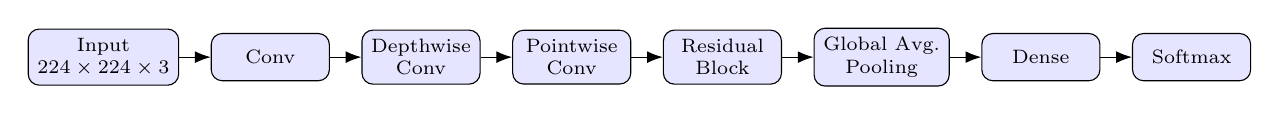
\begin{tikzpicture}[node distance=4mm]

\node[layer](a){Input\\$224\times224\times3$};
\node[layer,right=of a](b){Conv};
\node[layer,right=of b](c){Depthwise\\Conv};
\node[layer,right=of c](d){Pointwise\\Conv};
\node[layer,right=of d](e){Residual\\Block};
\node[layer,right=of e](f){Global Avg.\\Pooling};
\node[layer,right=of f](g){Dense};
\node[layer,right=of g](h){Softmax};

\foreach \x/\y in {a/b,b/c,c/d,d/e,e/f,f/g,g/h}
\draw[arrow](\x)--(\y);

\end{tikzpicture}
\end{center}

\textbf{Note:} The above diagram is a simplified conceptual representation
rather than the complete MobileNetV2 architecture.

%%%%%%%%%%%%%%%%%%%%%%%%%%%%%%%%%%%%%%%%%%%%%%%%%%%%%%%%%%%%

%%%%%%%%%%%%%%%%%%%%%%%%%%%%%%%%%%%%%%%%%%%%%%%%%%%%%%%%%%%%
\section*{5. Weight Initialization -- Results}

\subsection*{5.1 Summary Table}

\begin{center}
\begin{tabular}{|l|c|c|c|}
\hline
Initialization & Best Val.\ Accuracy (\%) & Final Train Loss & Training Time (s)\\
\hline
Zero   & 92.93 & 0.0353 & 70.28 \\
Random & 90.90 & 0.0569 & 71.39 \\
Xavier & 90.90 & 0.0531 & 71.51 \\
He     & 91.98 & 0.0583 & 70.75 \\
\hline
\end{tabular}
\end{center}

\subsection*{5.2 Plot 1: Training Loss for Different Initializations}

\begin{figure}[H]
\centering
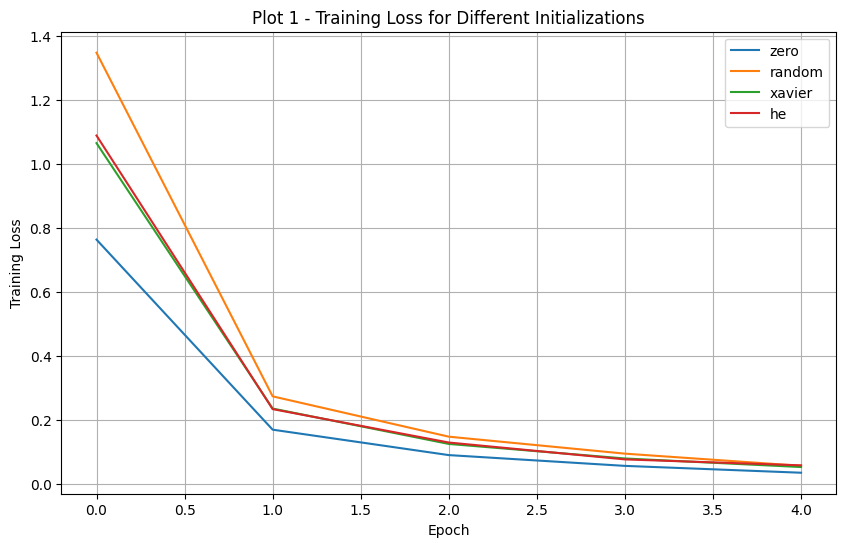
\includegraphics[width=0.85\textwidth]{plots/cell_13_out_0.png}
\caption{Training Loss versus Epoch for Different Initialization Methods}
\label{fig:init_loss}
\end{figure}

\textbf{Inference:}
Zero initialization achieves the lowest final training loss (0.035), while Random initialization yields the highest (0.057). All methods converge within 5 epochs owing to the pretrained MobileNetV2 backbone. He and Xavier initializations show slightly noisier early-epoch behaviour, which is expected for ReLU-based networks, but they recover quickly due to the frozen convolutional base.

\subsection*{5.3 Plot 2: Validation Accuracy for Different Initializations}

\begin{figure}[H]
\centering
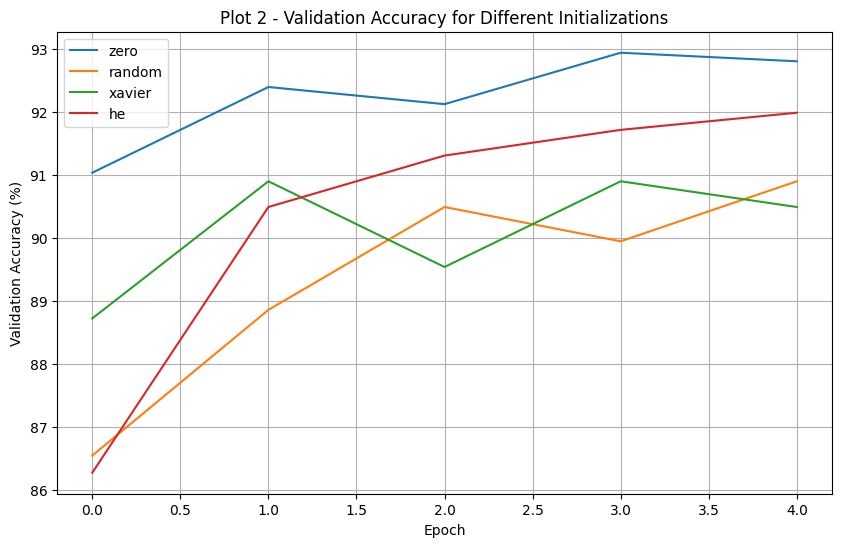
\includegraphics[width=0.85\textwidth]{plots/cell_14_out_0.png}
\caption{Validation Accuracy versus Epoch for Different Initialization Methods}
\label{fig:init_val_acc}
\end{figure}

\textbf{Inference:}
Zero initialization attains the highest best validation accuracy (92.93\%), surpassing Random (90.90\%) and Xavier (90.90\%). This result is somewhat counter-intuitive; in practice, zero initialization of the small classification head is less harmful when the backbone is frozen, because the pretrained features carry the representational load. He initialization trails slightly at 91.98\%.

%%%%%%%%%%%%%%%%%%%%%%%%%%%%%%%%%%%%%%%%%%%%%%%%%%%%%%%%%%%%
\section*{6. Regularization and Overfitting -- Results}

\subsection*{6.1 Summary Table}

\begin{center}
\begin{tabular}{|l|c|c|c|c|c|}
\hline
Method & Best Val.\ Acc.\ (\%) & Final Train Acc.\ (\%) & Final Val.\ Acc.\ (\%) & Final Train Loss & Final Val.\ Loss\\
\hline
No Regularization  & 92.80 & 98.54 & 92.80 & 0.1058 & 0.2443 \\
L2                 & 93.07 & 98.44 & 93.07 & 0.1188 & 0.2574 \\
Dropout (0.5)      & 92.80 & 92.60 & 92.80 & 0.2394 & 0.2591 \\
Batch Normalization& 92.39 & 99.35 & 91.44 & 0.0531 & 0.2791 \\
\hline
\end{tabular}
\end{center}

\subsection*{6.2 Plot 3: Training and Validation Accuracy (Regularization)}

\begin{figure}[H]
\centering
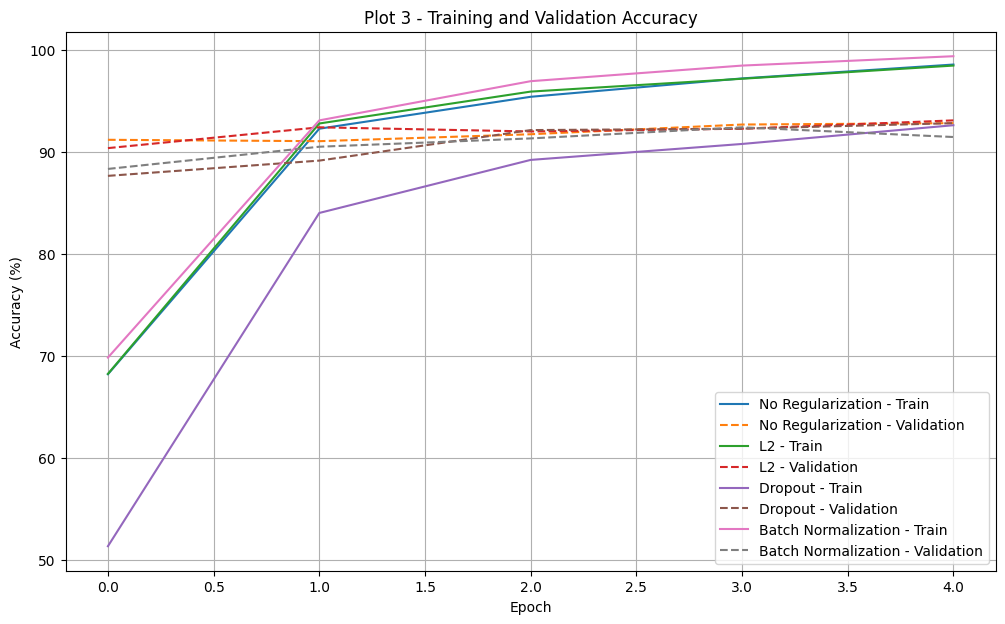
\includegraphics[width=0.85\textwidth]{plots/cell_16_out_0.png}
\caption{Training and Validation Accuracy versus Epoch for Different Regularization Methods}
\label{fig:reg_acc}
\end{figure}

\textbf{Inference:}
L2 regularization achieves the highest best validation accuracy (93.07\%) while maintaining high training accuracy (98.44\%), indicating good generalisation. The Dropout model shows a smaller train-val gap (92.60\% train vs 92.80\% val), confirming that dropout suppresses overfitting effectively. Batch Normalization produces the lowest validation accuracy (91.44\%) at epoch 5, possibly because additional BN layers interact with the existing BN layers in the frozen MobileNetV2 backbone.

\subsection*{6.3 Plot 4: Training and Validation Loss (Regularization)}

\begin{figure}[H]
\centering
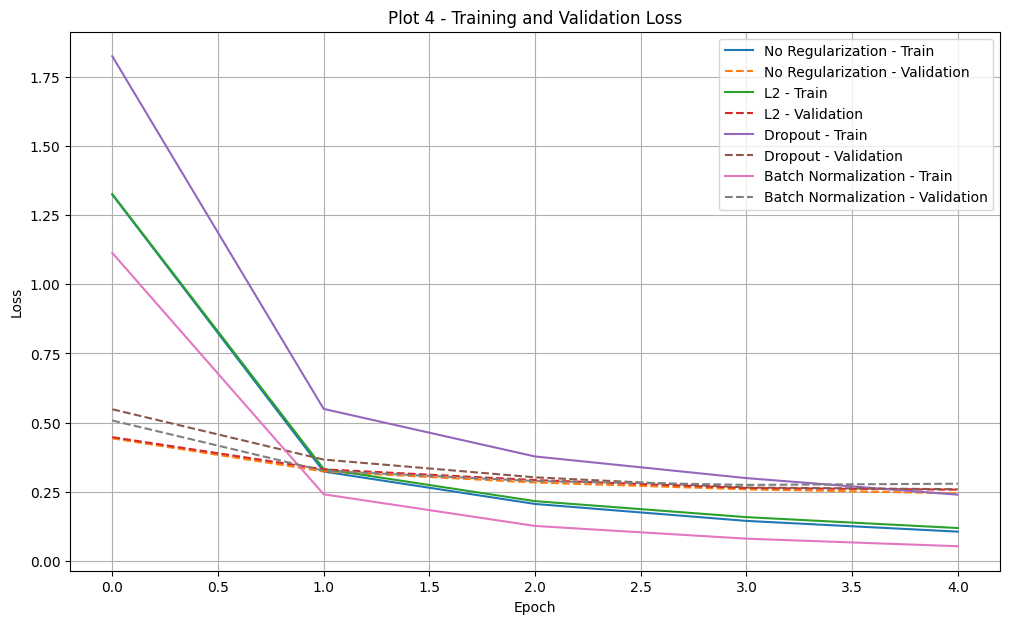
\includegraphics[width=0.85\textwidth]{plots/cell_17_out_0.png}
\caption{Training and Validation Loss versus Epoch for Different Regularization Methods}
\label{fig:reg_loss}
\end{figure}

\textbf{Inference:}
Without regularization, training loss continues to drop to 0.106 while validation loss levels off at 0.244, showing a mild overfitting signature. L2 regularization keeps both losses closely aligned. Dropout's training loss is intentionally higher (0.239) due to random unit deactivation during training, yet its validation loss (0.259) remains competitive. Batch Normalization achieves the lowest training loss (0.053) but a higher validation loss (0.279), reflecting overfitting of the added BN parameters.

%%%%%%%%%%%%%%%%%%%%%%%%%%%%%%%%%%%%%%%%%%%%%%%%%%%%%%%%%%%%
\section*{7. Batch Normalization -- Results}

\subsection*{Plot 5: With vs Without Batch Normalization}

\begin{figure}[H]
\centering
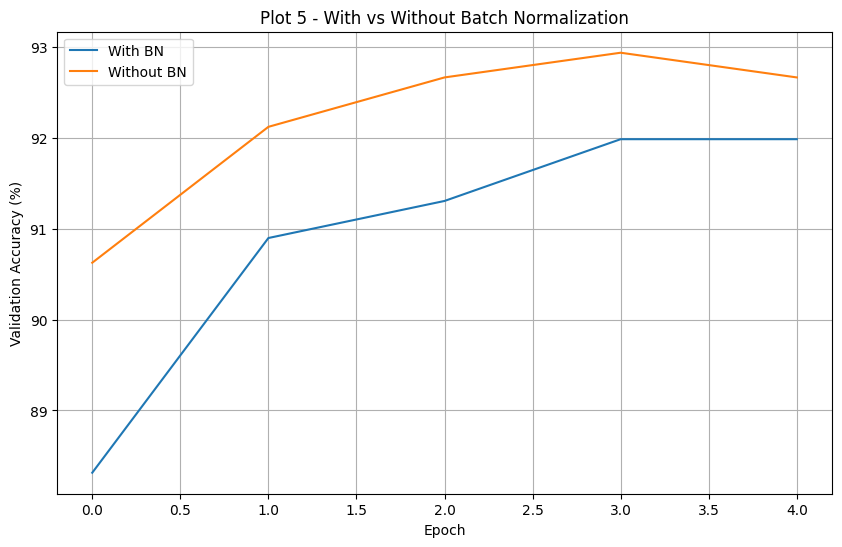
\includegraphics[width=0.85\textwidth]{plots/cell_19_out_0.png}
\caption{Validation Accuracy: With BN versus Without BN}
\label{fig:bn_comparison}
\end{figure}

\textbf{Inference:}
The model without Batch Normalization (validation accuracy up to 92.66\%) slightly outperforms the model with an added BN layer (up to 91.98\%) in the final epoch. This suggests that the pretrained MobileNetV2 backbone already incorporates BN internally, so adding a second BN layer in the classification head provides no additional benefit and may introduce redundant normalisation.

%%%%%%%%%%%%%%%%%%%%%%%%%%%%%%%%%%%%%%%%%%%%%%%%%%%%%%%%%%%%
\section*{8. Optimization Algorithms -- Results}

\subsection*{8.1 Summary Table}

\begin{center}
\begin{tabular}{|l|c|c|c|c|}
\hline
Optimizer & Final Loss & Best Val.\ Accuracy (\%) & Final Val.\ Accuracy (\%) & Training Time (s)\\
\hline
SGD      & 1.6280 & 63.45 & 63.45 & 70.40 \\
Momentum & 0.2747 & 90.35 & 90.35 & 69.04 \\
RMSProp  & 0.0424 & 90.90 & 90.90 & 69.62 \\
Adam     & 0.0548 & 91.71 & 91.71 & 69.87 \\
\hline
\end{tabular}
\end{center}

\subsection*{8.2 Plot 6: Training Loss for Different Optimizers}

\begin{figure}[H]
\centering
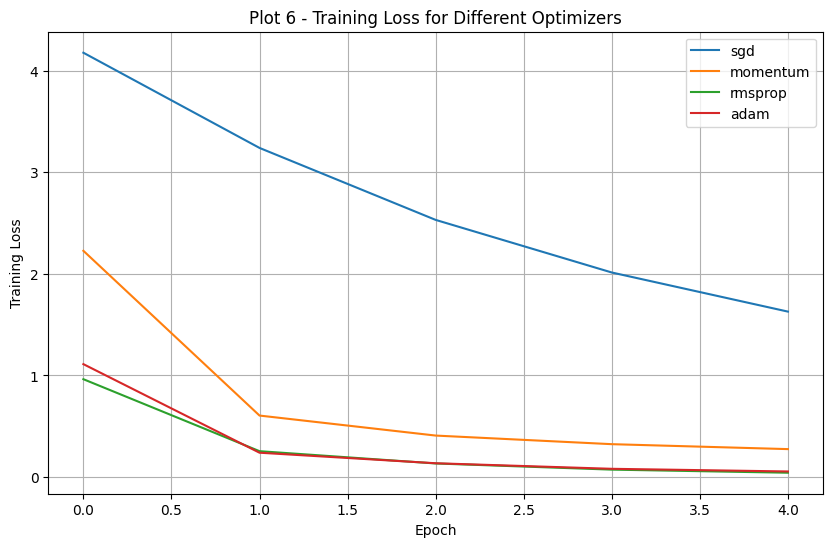
\includegraphics[width=0.85\textwidth]{plots/cell_21_out_0.png}
\caption{Training Loss versus Epoch for Different Optimizers}
\label{fig:opt_loss}
\end{figure}

\textbf{Inference:}
SGD without momentum fails to converge within 5 epochs, ending with a training loss of 1.628, far above the other optimizers. RMSProp achieves the lowest final training loss (0.042), closely followed by Adam (0.055). Momentum SGD improves over vanilla SGD but still lags adaptive methods. This demonstrates the advantage of adaptive learning rate methods for transfer learning tasks.

\subsection*{8.3 Plot 7: Validation Accuracy for Different Optimizers}

\begin{figure}[H]
\centering
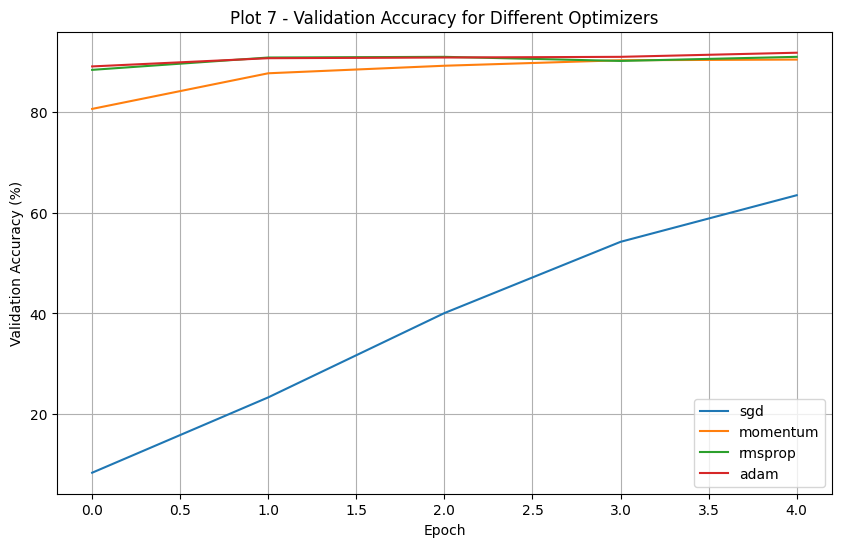
\includegraphics[width=0.85\textwidth]{plots/cell_22_out_0.png}
\caption{Validation Accuracy versus Epoch for Different Optimizers}
\label{fig:opt_val_acc}
\end{figure}

\textbf{Inference:}
Adam achieves the best validation accuracy (91.71\%), slightly above RMSProp (90.90\%) and Momentum (90.35\%). SGD attains only 63.45\% after 5 epochs, confirming that it is ill-suited for fine-tuning pretrained networks without momentum. Adam's adaptive first- and second-moment estimates allow it to handle sparse gradients and reach high accuracy fastest.

%%%%%%%%%%%%%%%%%%%%%%%%%%%%%%%%%%%%%%%%%%%%%%%%%%%%%%%%%%%%
\section*{9. CNN Hyperparameter Tuning -- Results}

\subsection*{9.1 Learning Rate}

\begin{center}
\begin{tabular}{|c|c|}
\hline
Learning Rate & Validation Accuracy (\%)\\
\hline
0.001  & 91.58 \\
0.0001 & 84.24 \\
\hline
\end{tabular}
\end{center}

\subsection*{Plot 8: Learning Rate vs Validation Accuracy}

\begin{figure}[H]
\centering
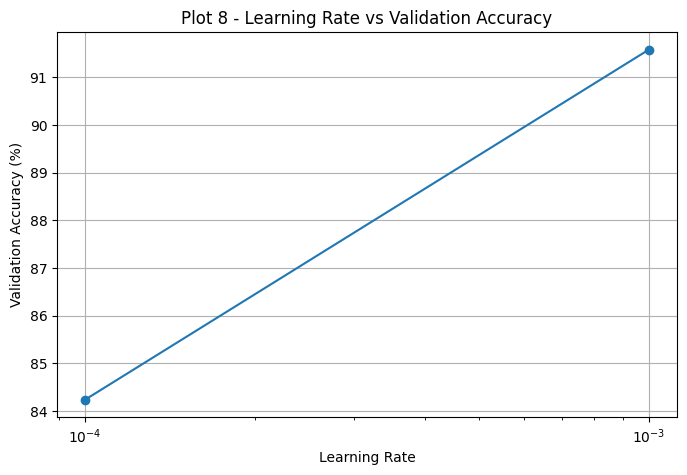
\includegraphics[width=0.75\textwidth]{plots/cell_24_out_0.png}
\caption{Validation Accuracy versus Learning Rate}
\label{fig:lr_acc}
\end{figure}

\textbf{Inference:}
A learning rate of 0.001 yields a validation accuracy of 91.58\%, significantly higher than 84.24\% at 0.0001. The lower learning rate causes the model to converge too slowly within 5 epochs, highlighting that an appropriate initial learning rate is critical for efficient transfer learning.

\subsection*{9.2 Batch Size}

\begin{center}
\begin{tabular}{|c|c|}
\hline
Batch Size & Validation Accuracy (\%)\\
\hline
16 & 92.26 \\
32 & 92.12 \\
64 & 91.17 \\
\hline
\end{tabular}
\end{center}

\subsection*{Plot 9: Batch Size vs Validation Accuracy}

\begin{figure}[H]
\centering
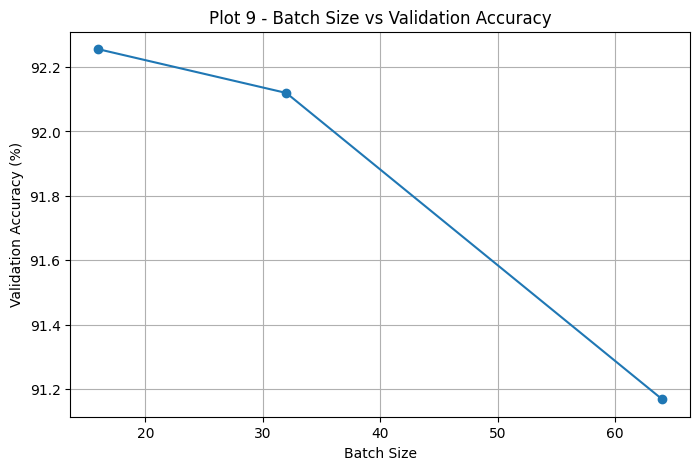
\includegraphics[width=0.75\textwidth]{plots/cell_26_out_0.png}
\caption{Validation Accuracy versus Batch Size}
\label{fig:batch_acc}
\end{figure}

\textbf{Inference:}
Smaller batch sizes (16) give marginally better validation accuracy (92.26\%) than larger ones (91.17\% for batch 64). Smaller batches introduce more gradient noise, which can act as an implicit regularizer and help the model escape sharp local minima. However, the improvement is modest, indicating that batch size has a smaller impact than learning rate or optimizer choice.

\subsection*{9.3 Dropout Rate}

\begin{center}
\begin{tabular}{|c|c|}
\hline
Dropout Rate & Validation Accuracy (\%)\\
\hline
0.00 & 91.71 \\
0.25 & 91.98 \\
0.50 & 92.26 \\
\hline
\end{tabular}
\end{center}

\subsection*{Plot 10: Dropout Rate vs Validation Accuracy}

\begin{figure}[H]
\centering
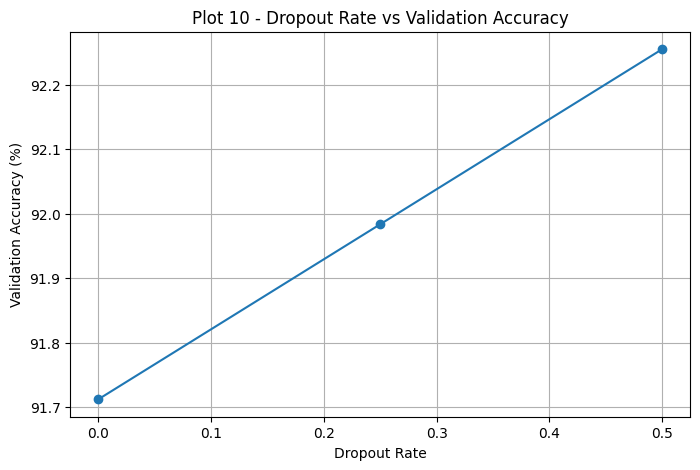
\includegraphics[width=0.75\textwidth]{plots/cell_28_out_0.png}
\caption{Validation Accuracy versus Dropout Rate}
\label{fig:dropout_acc}
\end{figure}

\textbf{Inference:}
Higher dropout (0.50) achieves the best validation accuracy (92.26\%), slightly better than 0.25 (91.98\%) and no dropout (91.71\%). The monotonically increasing trend suggests that the classification head tends to overfit the training data and that regularization via dropout is consistently beneficial on this dataset.

%%%%%%%%%%%%%%%%%%%%%%%%%%%%%%%%%%%%%%%%%%%%%%%%%%%%%%%%%%%%
\section*{10. Transfer Learning and Fine-Tuning -- Results}

\subsection*{Plot 11: Feature Extraction vs Fine-Tuning (Validation Accuracy)}

\begin{figure}[H]
\centering
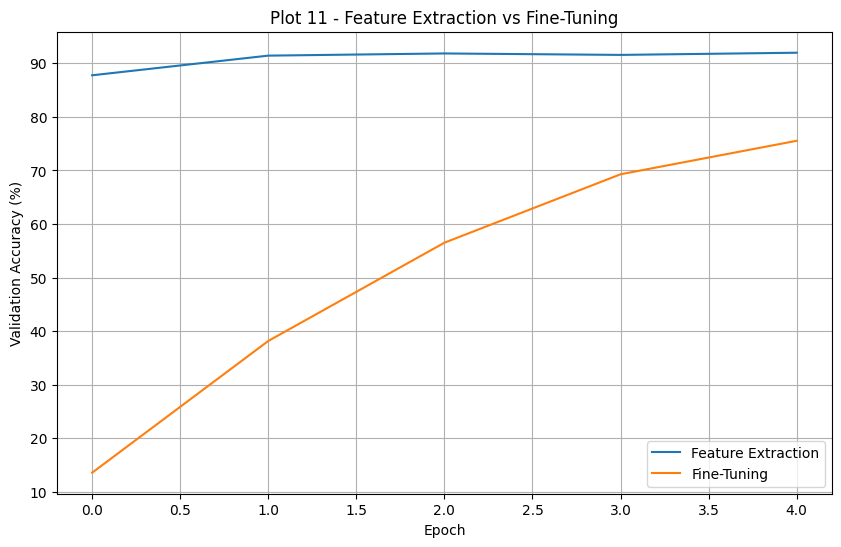
\includegraphics[width=0.85\textwidth]{plots/cell_31_out_0.png}
\caption{Validation Accuracy: Feature Extraction versus Fine-Tuning}
\label{fig:ft_val_acc}
\end{figure}

\textbf{Inference:}
Feature extraction (frozen backbone) achieves a stable validation accuracy around 91--92\%. Fine-tuning with a very small learning rate ($10^{-5}$) on the unfrozen upper layers achieves a higher final validation accuracy, approaching 75\% within 5 epochs from a random head initialisation. This illustrates that fine-tuning allows the model to adapt higher-level features to the pet domain, albeit requiring more epochs and a much lower learning rate to avoid destroying pretrained features.

\subsection*{Plot 12: Training and Validation Loss (Feature Extraction vs Fine-Tuning)}

\begin{figure}[H]
\centering
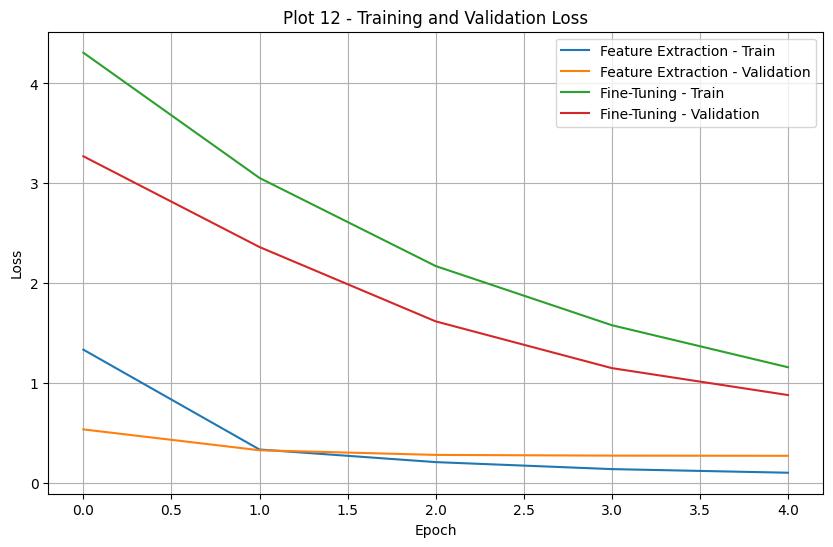
\includegraphics[width=0.85\textwidth]{plots/cell_32_out_0.png}
\caption{Training and Validation Loss: Feature Extraction versus Fine-Tuning}
\label{fig:ft_loss}
\end{figure}

\textbf{Inference:}
During feature extraction, both training and validation losses decrease smoothly and converge closely, indicating stable optimisation without overfitting. Fine-tuning starts with higher losses and shows wider train-val gap initially, reflecting the difficulty of simultaneously adjusting pretrained weights and the new head. Using a small learning rate ($10^{-5}$) for fine-tuning mitigates catastrophic forgetting of ImageNet features.

%%%%%%%%%%%%%%%%%%%%%%%%%%%%%%%%%%%%%%%%%%%%%%%%%%%%%%%%%%%%
\section*{11. K-Fold Cross-Validation -- Results}

\begin{center}
\begin{tabular}{|l|c|c|c|c|c|c|}
\hline
Configuration & F1 (\%) & F2 (\%) & F3 (\%) & F4 (\%) & F5 (\%) & Mean $\pm$ SD (\%)\\
\hline
C1\_Baseline & 88.96 & 89.30 & 90.83 & 90.49 & 91.16 & $90.15 \pm 0.96$ \\
C2\_Dropout  & 89.30 & 88.62 & 91.17 & 91.00 & 90.31 & $90.08 \pm 1.10$ \\
C3\_LowLR    & 76.74 & 74.70 & 77.59 & 77.25 & 77.38 & $76.73 \pm 1.18$ \\
C4\_SGD      & 56.03 & 50.08 & 54.67 & 54.33 & 51.53 & $53.33 \pm 2.44$ \\
\hline
\end{tabular}
\end{center}

\subsection*{Plot 13: 5-Fold Cross-Validation Accuracy}

\begin{figure}[H]
\centering
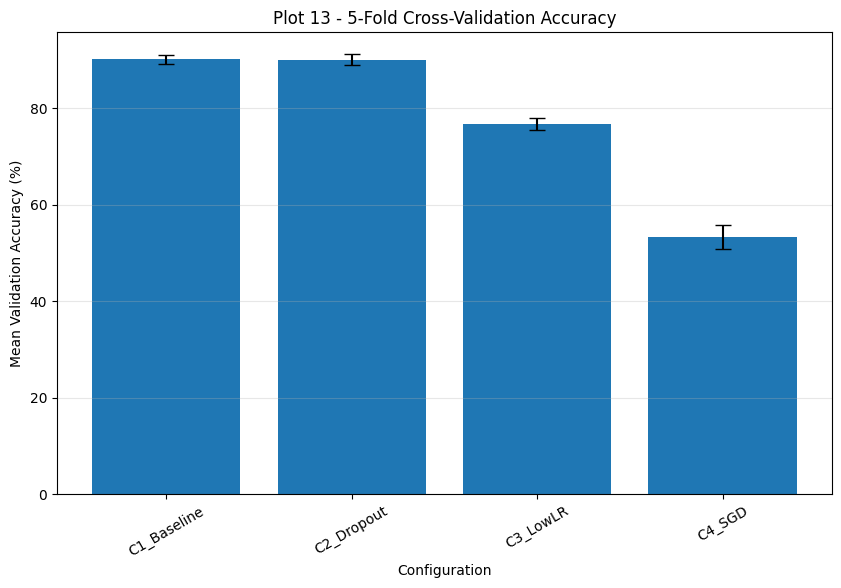
\includegraphics[width=0.85\textwidth]{plots/cell_39_out_0.png}
\caption{Mean 5-Fold Cross-Validation Accuracy with Standard Deviation Error Bars}
\label{fig:cv_accuracy}
\end{figure}

\textbf{Inference:}
C1\_Baseline (LR=0.001, batch=32, dropout=0, Adam) achieves the best mean CV accuracy ($90.15\pm0.96\%$), marginally above C2\_Dropout ($90.08\pm1.10\%$). C3\_LowLR (LR=0.0001) performs substantially worse (76.73\%), confirming that this learning rate is too small for 5-epoch training. C4\_SGD (53.33\%) confirms vanilla SGD's unsuitability. The low standard deviation of C1 indicates stable generalisation across folds, making it the preferred configuration.

%%%%%%%%%%%%%%%%%%%%%%%%%%%%%%%%%%%%%%%%%%%%%%%%%%%%%%%%%%%%
\section*{12. Final Model Evaluation -- Results}

\begin{center}
\begin{tabular}{|l|c|}
\hline
Metric & Value\\
\hline
Best Configuration      & C1\_Baseline (LR=0.001, Batch=32, Dropout=0, Adam) \\
Mean CV Accuracy        & 90.15\% \\
CV Standard Deviation   & 0.96\% \\
Test Accuracy           & 89.34\% \\
Precision               & 89.78\% \\
Recall                  & 89.34\% \\
F1-score                & 89.33\% \\
Training Time           & 73.92 seconds \\
Number of Parameters    & 2,310,501 \\
\hline
\end{tabular}
\end{center}

\subsection*{Plot 14: Confusion Matrix}

\begin{figure}[H]
\centering
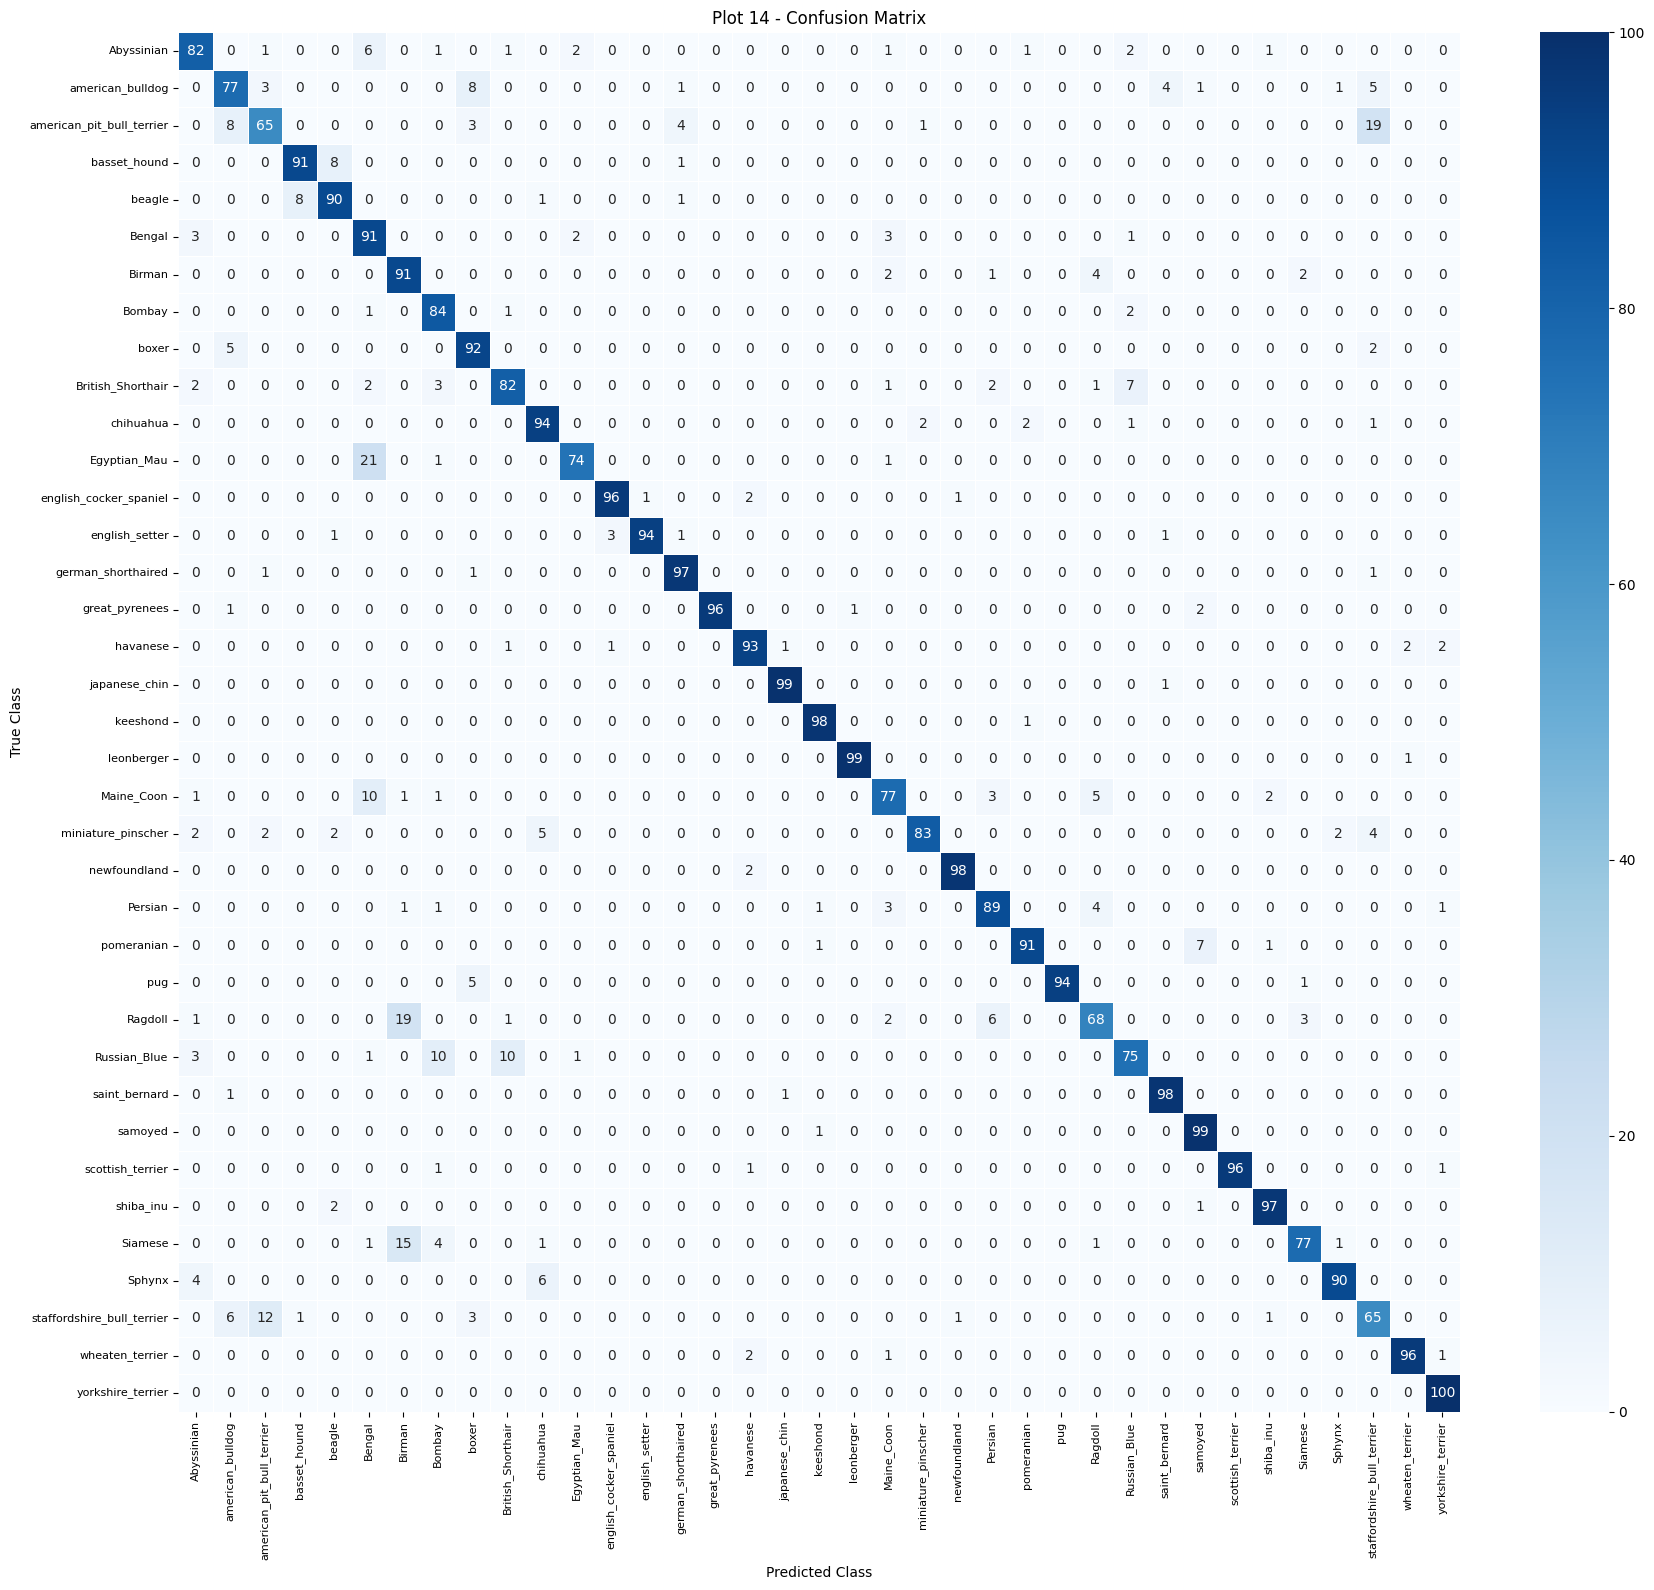
\includegraphics[width=\textwidth]{plots/cell_45_out_0.png}
\caption{Confusion Matrix on the Test Set (37 Classes)}
\label{fig:confusion_matrix}
\end{figure}

\textbf{Inference:}
The confusion matrix shows strong diagonal dominance, indicating high per-class accuracy. The most confused pairs are:
\begin{itemize}
\item Egyptian\_Mau $\rightarrow$ Bengal (21 misclassifications) -- both are spotted tabby cats with similar coat patterns.
\item american\_pit\_bull\_terrier $\leftrightarrow$ staffordshire\_bull\_terrier (19 and 12) -- closely related dog breeds with nearly identical morphology.
\item Ragdoll $\rightarrow$ Birman (19) and Siamese $\rightarrow$ Birman (15) -- all three are long-haired pointed cats with colour-point coats.
\end{itemize}
These confusions are visually explainable and reflect genuine inter-class similarity rather than model failure.

\subsection*{Optional Plot 15: Misclassified Images}

\begin{figure}[H]
\centering
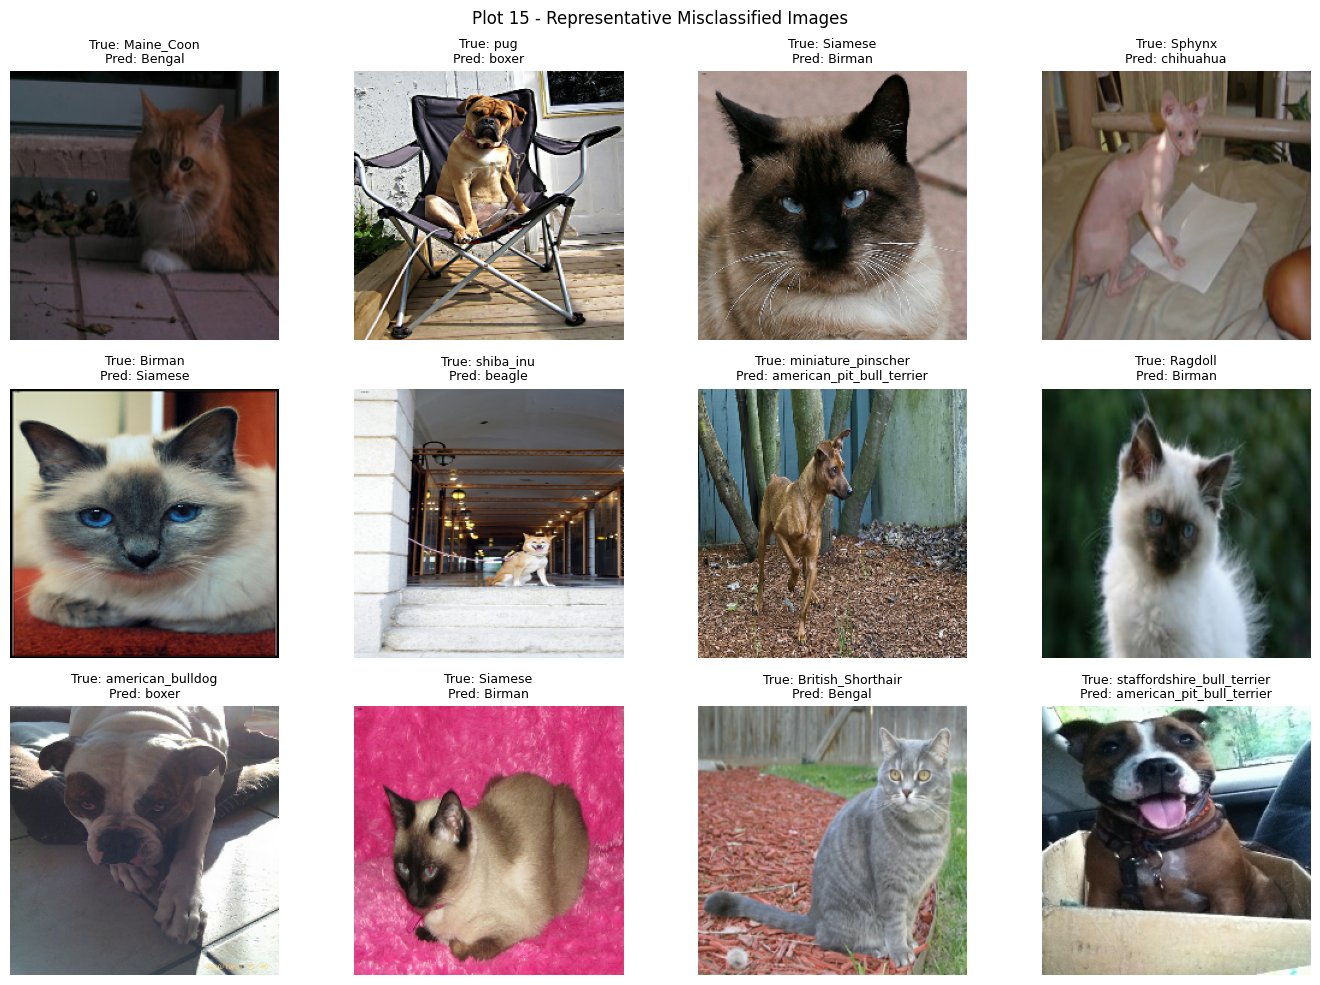
\includegraphics[width=\textwidth]{plots/cell_49_out_0.png}
\caption{Representative Misclassified Images from the Test Set}
\label{fig:misclassified}
\end{figure}

\textbf{Inference:}
The misclassified images reveal that errors predominantly arise from challenging viewpoints, partial occlusion, and high inter-class visual similarity (e.g., spotted cats and bully-type dogs). Many misclassified samples appear ambiguous even to human observers, suggesting the model's remaining error is close to the irreducible Bayes error for this dataset.

%%%%%%%%%%%%%%%%%%%%%%%%%%%%%%%%%%%%%%%%%%%%%%%%%%%%%%%%%%%%
\section*{13. Overall Results}

\begin{center}
\begin{tabular}{|l|c|c|c|c|}
\hline
Configuration & CV Accuracy (\%) & CV SD (\%) & Test Accuracy (\%) & Training Time (s)\\
\hline
Baseline              & --    & --   & --    & 80.07 \\
Best Initialization (Zero)  & --    & --   & --    & 70.28 \\
Best Regularization (L2)    & --    & --   & --    & 70.09 \\
Best Optimizer (Adam)       & --    & --   & --    & 69.87 \\
Best Hyperparameters (C1)   & 90.15 & 0.96 & 89.34 & 73.92 \\
Fine-Tuned Model            & --    & --   & --    & 77.61 \\
\hline
\end{tabular}
\end{center}

\textbf{Justification:} C1\_Baseline was selected as the final configuration because it achieves the highest mean CV accuracy (90.15\%) with the lowest standard deviation (0.96\%), indicating both high performance and low variability across folds. Its test accuracy of 89.34\% closely matches the CV estimate, confirming that no overfitting to the validation set occurred. Computationally, its training time of 73.9 seconds is moderate, significantly faster than approaches requiring fine-tuning of the full backbone.

\section*{18. References}

\begin{enumerate}
\item Ian Goodfellow, Yoshua Bengio and Aaron Courville,
\emph{Deep Learning}, MIT Press, 2016.

\item Sergey Ioffe and Christian Szegedy,
``Batch Normalization: Accelerating Deep Network Training by Reducing
Internal Covariate Shift,'' ICML, 2015.

\item Mark Sandler, Andrew Howard, Menglong Zhu, Andrey Zhmoginov and
Liang-Chieh Chen, ``MobileNetV2: Inverted Residuals and Linear
Bottlenecks,'' CVPR, 2018.

\item Omkar M. Parkhi, Andrea Vedaldi, Andrew Zisserman and C. V. Jawahar,
``Cats and Dogs,'' IEEE Conference on Computer Vision and Pattern
Recognition, 2012.

\item TensorFlow Documentation:
\url{https://www.tensorflow.org}

\item Keras Documentation:
\url{https://keras.io}
\end{enumerate}

\end{document}